%! suppress = LineBreak
%! suppress = MissingLabel
%! suppress = FileNotFound
\documentclass[../main.tex]{subfiles}

\begin{document}

    \subsubsection{Model maszyny stanowej}

    \textbf{Testowanie maszyny stanowej}
    \begin{itemize}
        \item \textbf{reprezentacja możliwych stanów systemu i przejść między nimi}
        \item metoda \textbf{opisu dynamiki} systemu
    \end{itemize}

    \begin{table}[H]
        \begin{center}
            \begin{tabular}{ p{6cm} p{10cm}}
                \textbf{n-switch coverage} - pokrycie przejść o \textbf{n} stanach pomiędzy stanem początkowym i końcowym.
                Żeby zidentyfikować pokrycie n-switchy zidentyfikuj wszystkie (n-1)-switche i ich rozszerzenia.
                &
                \raisebox{-\totalheight}{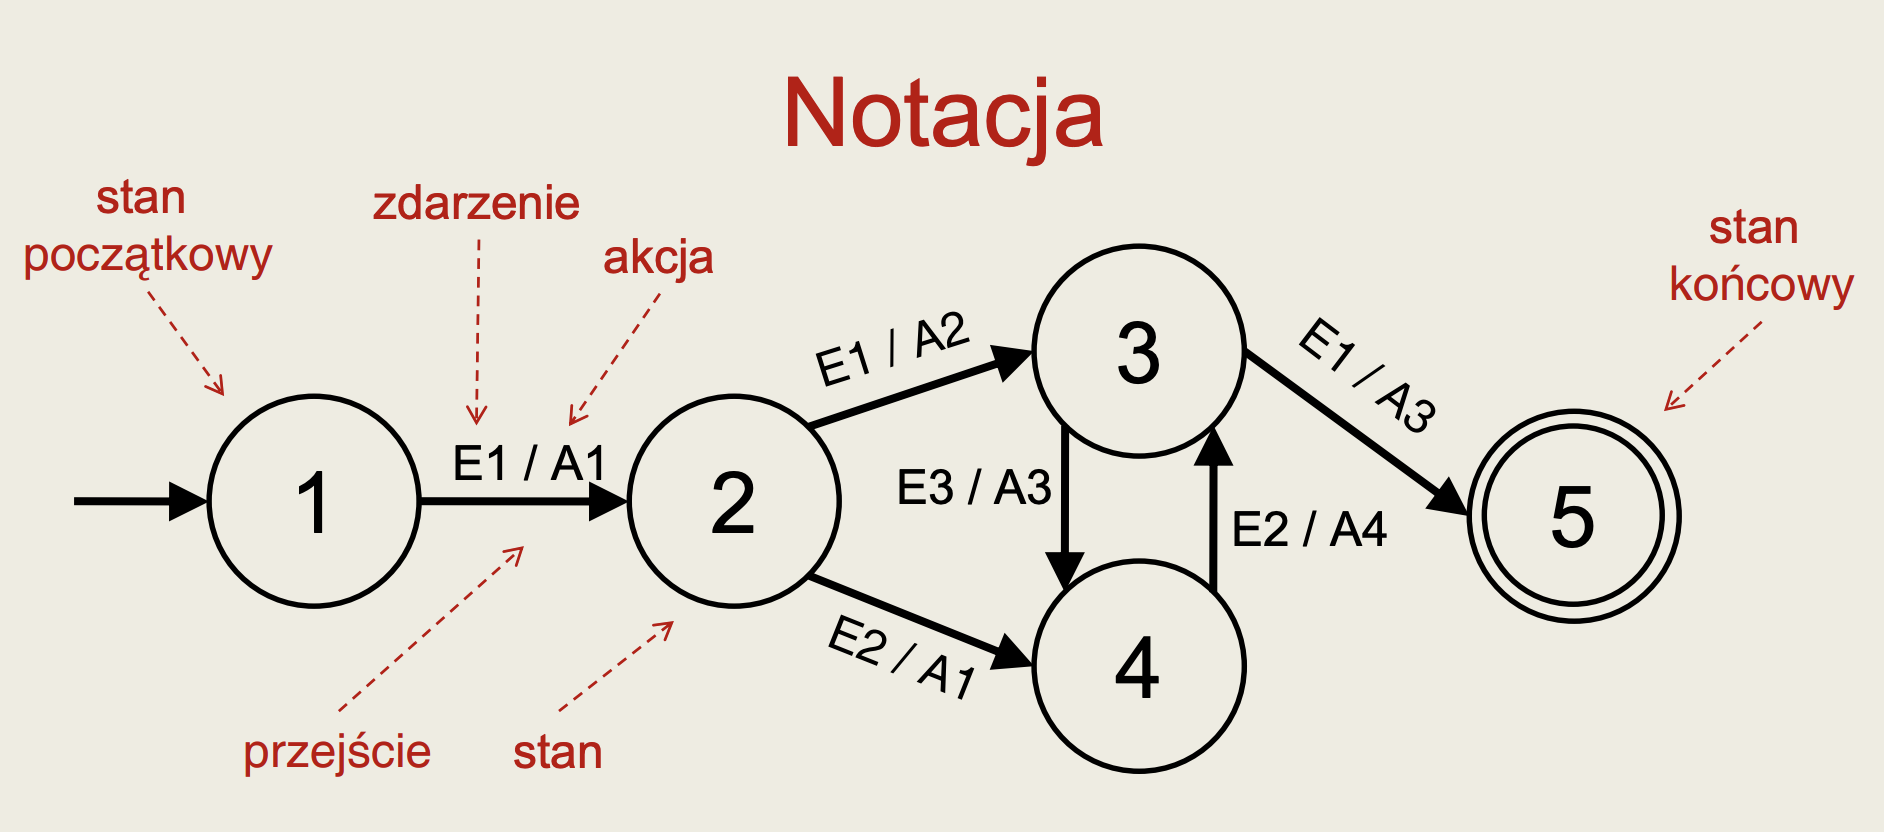
\includegraphics[width=10cm]{maszyna.png}}\\
            \end{tabular}
        \end{center}
    \end{table}

    \subsubsection{Drzewa klasyfikacji}

    \begin{table}[H]
        \begin{center}
            \begin{tabular}{ p{8cm} p{8cm}}
                \begin{itemize}
                    \item szczególna wersja metody \textbf{Category-Partition}
                    \item graficzna reprezentacja systemu jako:
                    \begin{itemize}
                        \item zestawu \textbf{cech}
                        \item ich \textbf{wartości}
                        \item ewentualnych \textbf{związków} między wartościami cech
                    \end{itemize}
                \end{itemize}

                &
                \begin{itemize}
                    \item odmiana metody: \textbf{model cech} (ang. feature model)
                    \item wykorzystywany jako model w podejściu SPL (Software Product Lines)
                    \item wyprowadzanie testów wykorzystuje zwykle jedno z podejść
                    kombinacyjnych
                \end{itemize}

            \end{tabular}
        \end{center}
    \end{table}

    \begin{figure}[H]
        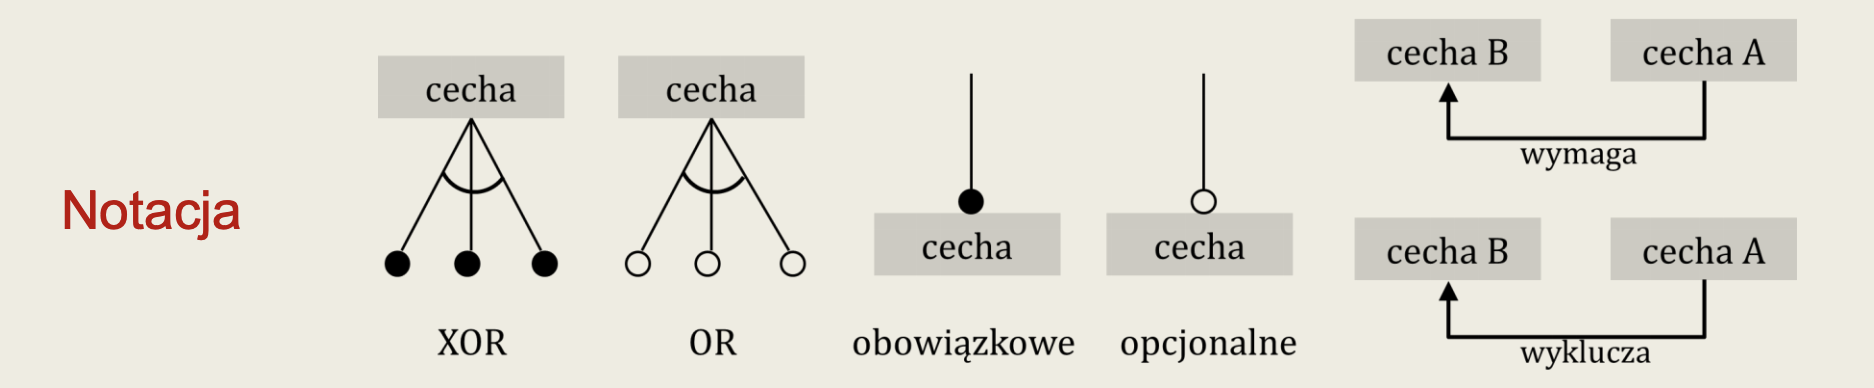
\includegraphics[width=\linewidth]{drzewa.png}
    \end{figure}

    \subsubsection{Testowanie kombinatoryczne}
    \begin{itemize}
        \item stosowane gdy chcemy testować \textbf{kombinacje klas równoważności}
        różnych podziałów
        \item metody kombinatoryczne pozwalają na redukcję liczby testów
    \end{itemize}

    \textbf{Pełne pokrycie kombinatoryczne} = każda kombinacja klas wszystkich podziałów.

    \textbf{1-wise, Each Choice} = każda klasa z każdego podziału ma być przetestowana przynajmniej raz.
    Liczba kombinacji = max ilości klas.

    \textbf{2-wise, Pairwise} = każda para klas z dowolnych dwóch podziałów musi wystąpić przynajmniej raz. Minimalna
    liczba kombinacji jest NP-zupełna.

    \subsubsection{Testowanie losowe}
    \begin{itemize}
        \item wymaga możliwości \textbf{losowego wyboru elementu dziedziny}
        \item może być przeprowadzane manualnie, ale \textbf{zwykle automatyczne}
        \item można stosować, gdy trudno modelować dziedzinę wejściową
    \end{itemize}


    \begin{table}[H]
        \begin{center}
            \begin{tabular}{ p{8cm} | p{8cm}}
                \textbf{Automatyzacja testowania losowego}.

                Pełna automatyzacja testowania losowego jest możliwa gdy:
                \begin{itemize}
                    \item można \textbf{automatyczne losować dane wejściowe}
                    \item można \textbf{automatycznie określać oczekiwane wyjście} lub automatycznie porównywać wyjście ze specyfikacją
                    \begin{itemize}
                        \item istnieje wyrocznia
                        \item interesuje nas tylko crash
                        \item łatwa weryfikacja wyjścia (sortowanie)
                        \item łatwo wygenerować wejście z wyjścia (np. pierwiastek/potęga)
                    \end{itemize}
                \end{itemize}

                &
                \raisebox{-\totalheight}{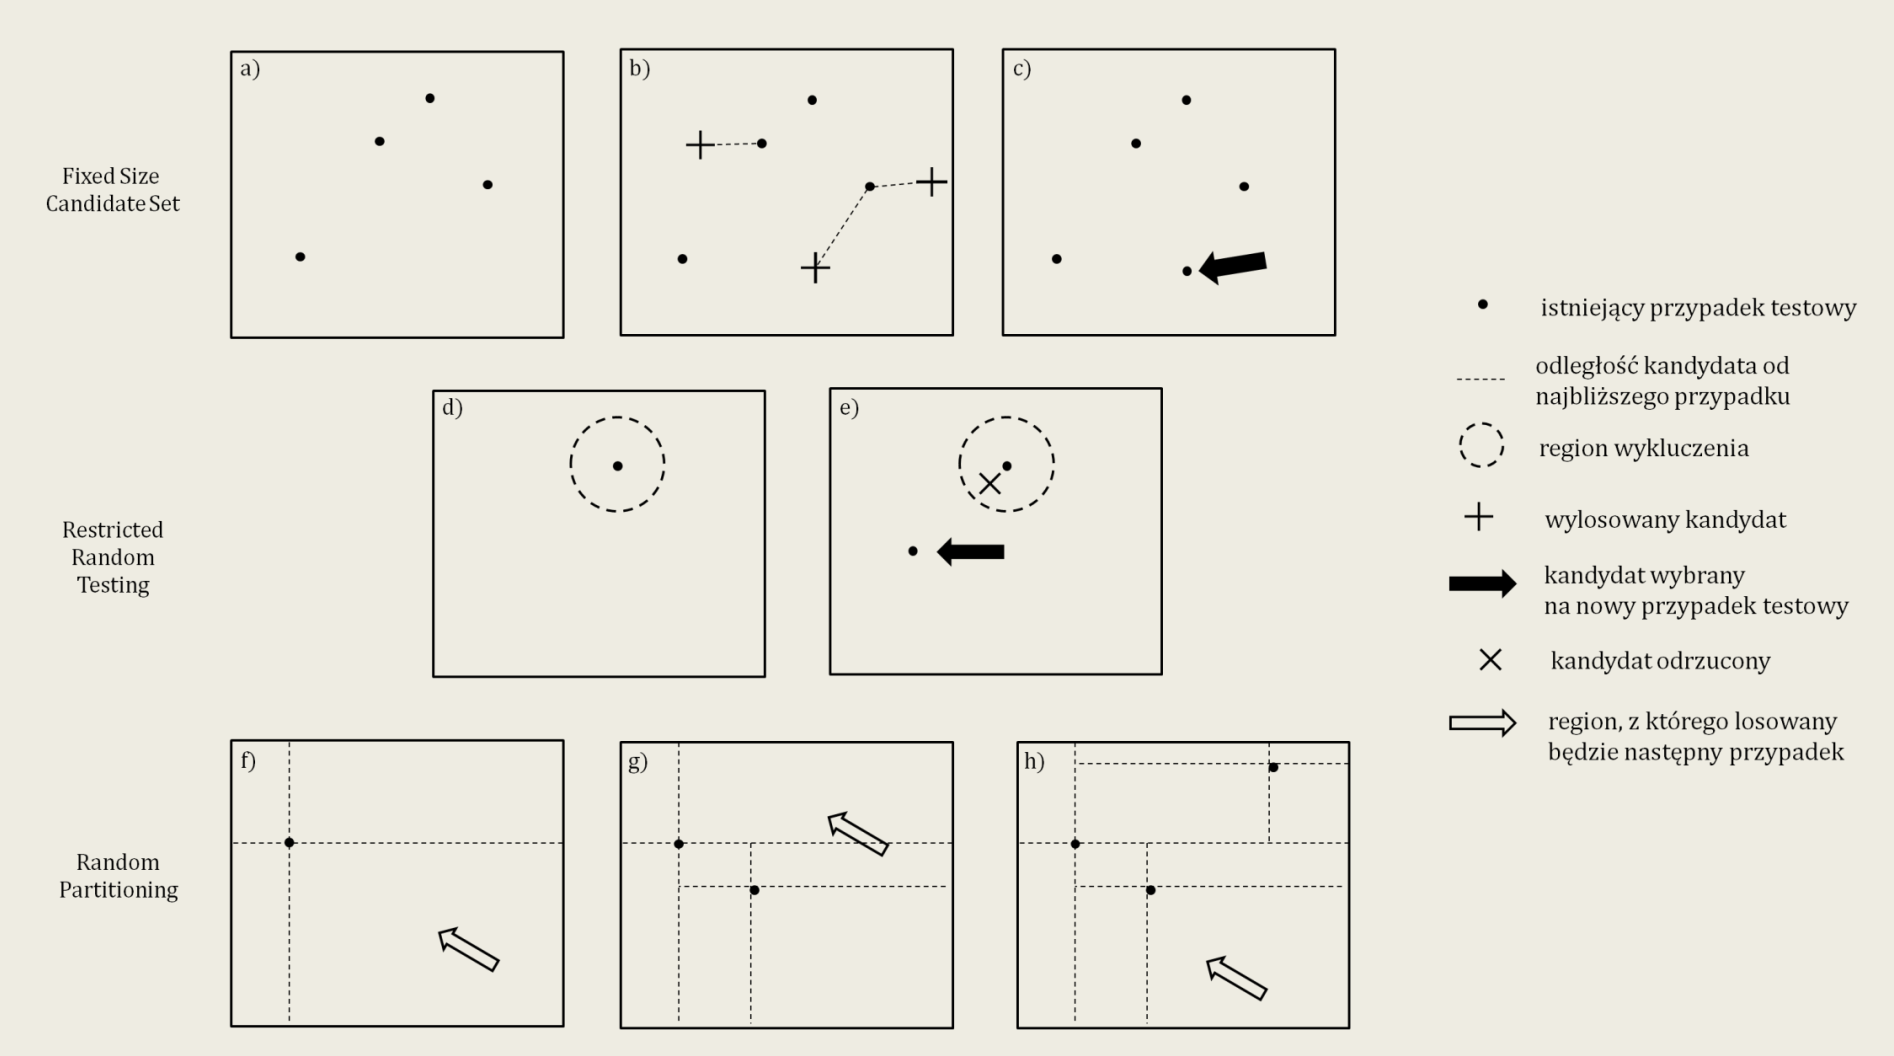
\includegraphics[width=\linewidth]{losowe.png}}
                \\
            \end{tabular}
        \end{center}
    \end{table}

    \subsubsection{Testowanie oparte na use-case'ach}
    \begin{itemize}
        \item przypadek użycia opisuje \textbf{interakcję użytkownika z systemem}
        \item zwykle \textbf{wysokopoziomowy}, w postaci przepływu „end-to-end”
        \item testowanie oparte na przypadkach użycia \textbf{sprawdza poprawność
        działania systemu dla przepływów}: głównego i alternatywnych
    \end{itemize}

    \textbf{Generowanie przypadków użycia:}
    \begin{enumerate}
        \item Dla każdego przypadku użycia wygeneruj \textbf{pełny zbiór scenariuszy}.
        \item Dla każdego scenariusza zidentyfikuj \textbf{przynajmniej 1 przypadek testowy} i warunki
        umożliwiające jego wykonanie.
        \item Dla każdego przypadku testowego zidentyfikuj \textbf{dane}, dla których można przeprowadzić test.
    \end{enumerate}

    \subsubsection{Testowanie CRUD}

    \begin{itemize}
        \item CRUD = \textbf{Create, Read, Update, Delete}
        \item metoda testowania \textbf{cyklu życia danych} (encji)
        \item cykl życia reprezentowany przy pomocy tzw. \textbf{macierzy CRUD}
        \begin{itemize}
            \item wiersze = funkcje, kolumny = encje, przecięcie = operacja
            \item dla każdej funkcji sprawdzamy które encje są wykorzystywane
            \item a następnie, które akcje (C, R, U, D) są na nich przeprowadzane
        \end{itemize}
        \item dwa rodzaje testów
        \begin{itemize}
            \item \textbf{sprawdzanie kompletności (statyczny)}
            \begin{itemize}
                \item sprawdzenie, czy \textbf{dla każdej encji występują wszystkie 4 operacje}
                \item brak jakiejś akcji niekoniecznie oznacza błąd w systemie, ale powód tego braku powinien zostać wyjaśniony
            \end{itemize}
            \item \textbf{sprawdzanie spójności (dynamiczny)}
            \begin{itemize}
                \item sprawdza \textbf{integrację różnych funkcji}
                \item przypadki testowe konstruujemy zadając cały cykl życia encji:
                \item każdy przypadek testowy zaczyna się od C i przechodzi do
                wszystkich możliwych U, kończąc na D; jeśli jest więcej możliwości
                C i D, tworzy się dodatkowe przypadki
                \item po każdej akcji (C, U, D) występuje jedno lub kilka R – to sprawdza,
                czy encja została poprawnie przetworzona i jest użyteczna dla innych funkcji
                \item dla każdej encji, wszystkie wystąpienia akcji (C, R, U i D) we
                wszystkich funkcjach powinny zostać pokryte przez przypadki testowe
            \end{itemize}
        \end{itemize}
    \end{itemize}
\end{document}
